\documentclass[11pt]{article}
\usepackage[small,compact]{titlesec}
\usepackage[margin=0.5in]{geometry}
\usepackage{common}
\usepackage{wrapfig}
\usepackage{subcaption}
\title{Practical 1: Predicting the Efficiency of Organic Photovoltaics\\Repository: https://github.com/tongbaojia/pubcs181}
\author{Baojia Tong, baojia.tong@cern.ch \\ Yuliya Dovzhenko, dovzhenko@g.harvard.edu \\ Alan Le Goallec, alanlegoallec@g.harvard.edu}
\begin{document}
\maketitle{}

\paragraph{Abstract}
We were asked to predict the suitability of 800K different molecules for use in solar panels. The relevant physical property of these molecules that we tried to predict was the "gap" value, defined by the difference in energy between the highest and the lowest occupied molecular orbital. The features that we used were all computed from the string representation of the molecule, using the RDkit package. We will first present how we preprocessed the data, and we will then describe the different machine algorithms that we used and the results we obtained.

\section{Technical Approach: Preprocessing}


  \subsection{Data Cleaning: Removing weakly correlated features}
\paragraph{}
    The samples that we were given contained 256 features precalculated using RDkit.
    \textbf{The first step was to check how many of these features contain significant information, and to remove weakly correlated features.}
    In theory, extra useless features should not prevent us from finding a good model, as they can easily
    be ignored if necessary. However,
    they can slow down the tuning process and keep us from exploring some models or some non linear
    feature transformations within a reasonable time. \textbf{To filter the features that we judged useless, we first looked at their correlation with the "gap" values, and got rid of every feature that was not at least 10\% correlated.}
    It appeared that the vast majority of the features were poorly correlated with our outcome of interest, or simply have the value of zero for all entries.
    %We are well aware that in theory a feature could have an impressive predictive power while showing a 0\% correlation with the output (for example if the correlation is +1 on half of the samples, and -1 with the other half, which a decision tree could exploit if these two halves can be separated using the value of one of the predictors), but we find it unlikely here and we are willing to take the risk to loose some information.
    After this first preprocessing step, we were left with only 7 predictors from the original 256 features.
    %Note: to save some time, we only used 20\% of the data to determine which features we should use.
\begin{figure}
\centering
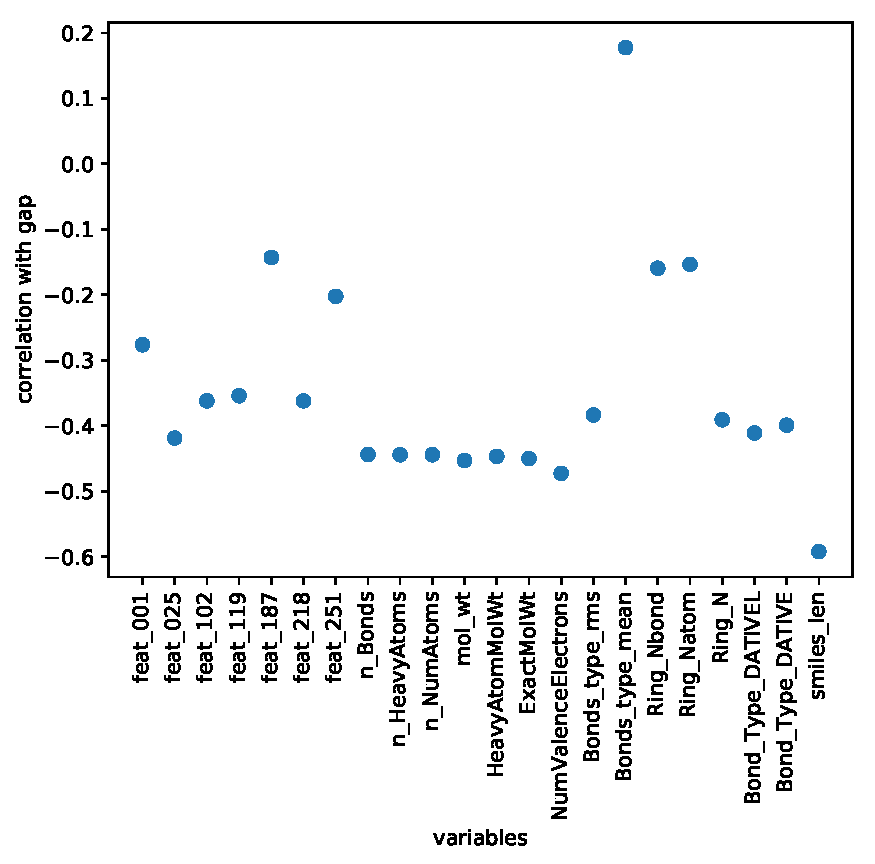
\includegraphics[width=0.2\textwidth]{Var-gap.pdf}
\caption{List of kept variables and their correlation with gap. Correlations are calculated using $20\%$ of the total training sample. Notice only features with $> 0.1$ correlation with gap are kept.}
\label{fig:var}
\end{figure}
  \subsection{Data Mining: Adding chemistry features with rdchem}
\paragraph{}
From basic quantum mechanics, there are tree kinds of information that will determine the gap: first, the degree of electron orbital overlap (bonds), second the size of the nuclei, and third the chemical potential level, which is related to the average number of electrons per atom. We found the following useful properties the rdkit Descriptor package: number of heavy atoms, number of atoms, molecular weight, average molecular weight of heavy atoms, average molecular weight, number of valence electrons and number of radical electrons. Also the bond information and ring information of the molecules were explored and utilised. The list of variables and their correlation is shown in Figure \ref{fig:var}. To see the effect, after adding new features, we compare the RMSE with benchmark training set and testing using an orthogonal subset of the training sample. For the same models, the results are significantly improved: 
\begin{itemize}
\item{Without extra features: LR RMSE = 0.3047;  RF RMSE = 0.2874}
\item{With descriptor extra features(no bond or ring yet) :LR RMSE = 0.2252;  RF RMSE = 0.2273}
\end{itemize}
  \paragraph{Some other notes:}
    \textbf{Adding nonlinear terms:} To capture the potential interactions between the different predictors, we added the interaction terms (the products between the different predictors). We also computed the quadratic terms. This was only a realistic idea because of the previous filtering of the not so useful features. \textbf{Scaling:} Gap value is by nature a float. Because the unit is arbitary, we scaled all the gap value by a factor of 1000. We made sure to do that by only looking at the training set, and then unapplied the same transformations to the columns of the testing set.
    
  \subsection{Data Splitting: Training and Testing samples}
\paragraph{}
    Because the there isn't a testing sample with gap value, the training dataset is chosen to be either $20\%$ or $80\%$ of the total training set, and from the orthogonal dataset $4\%$ or $16\%$ of the dataset is used a the testing dataset. More effort could be spent here but this is good enough for our testing.
    
\section{Technical Approach: Models}
    \subsection{Main model: Regularized Linear Regression}
    \paragraph{}
    We chose to first focus on Linear Regression, and regularized it in different ways. We used LASSO as a penalty: LASSO adds a regulariation term in norm 1, which encourages a sparse model: the total sum of the
    coefficients tends to remain small, but it does not matter how this quantity is spread between the features.
    So if some features are correlated, one of them will tend to carry the weight of the others and see its coefficient increase, while the 
    other features see their coefficient set to zero. 
    \paragraph{}
    We then used RIDGE regression: this time the penalty term is in norm 2, so big coefficients are even more penalized: not only is the sum
    of the coefficient encouraged to remain small, but individual coefficient tend to do the same. So if several features are
    correlated, the model will tend to distribute the total amount of coefficient between the features. Therefore the resulting model is not
    as sparse as the one generated by LASSO regression. 
    \paragraph{}
    Finally we used an elastic net. An elastic net is basically the combination between a LASSO and a RIDGE regression, since an extra
    hyperparameter is introduced: if this parameter is 0, the elastic net is equivalent to a LASSO. If this parameter is 1, it is equivalent
    to a RIDGE. For every value in between 0 and 1, the model is trying a weighted compromise between LASSO and RIDGE regularization.
    So an elastic net basically introduces an extra hyperparameter to do model selection between LASSO, RIDGE, and their combinations.
    
    \subsection{Partial Least Squares}
    \paragraph{}
Since we are dealing with a large sparse matrix (many zeros in the original features), we decided to explore dimension reduction. In particular, we focused on the Partial Least Squares (PLS) algorithm, which projects the data onto planes of greatest variance. These planes are referred to as principal components, and they represent the degree of variability that exists in the data. We have already seen in the Preprocessing section that not all features are equally important in predicting the data.
\paragraph{}
Our results are plotted in figure \ref{fig:PLS}.  The four plots correspond to PLS results different sets of data: (a) original data, (b) original data with additional chemistry features, and (c) truncated data with chemistry features, and (d) truncated data with additional features and polynomial terms. For comparison, all four tests were performed on the same subsets of the data, with 40,000 molecules used for training and 8,000 molecules used for testing. 
All four plots show the RMSE converging toward a minimum value, but the value of the RMSE plateau is different in different cases. With only original data, the error is ~0.3, comparable with the LR benchmark. This indicates to us that the features in the data can be accurately represented by a little over 10 components. However, the plateau in RMSE does not mean that we have found the optimal model. It merely indicates that there may be non-linear features present in the data, which we cannot identify with a principal component analysis. 
\begin{figure}[] 
\centering
\begin{subfigure}[!t]{0.2\textwidth}
        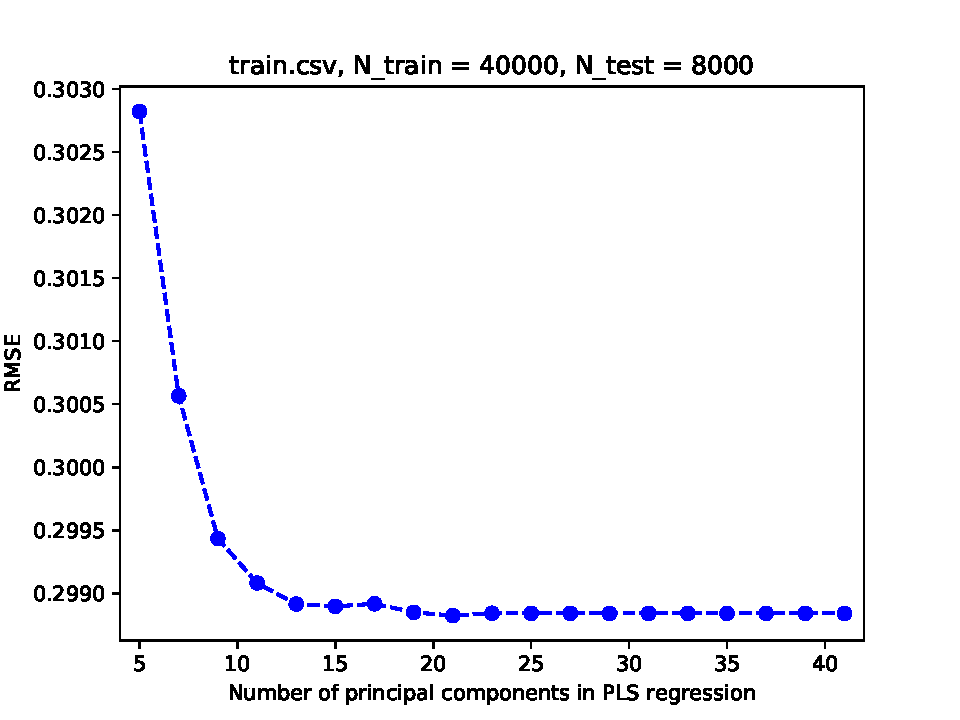
\includegraphics[width=\textwidth]{train_N_train_40000_N_test_8000.pdf}
    \end{subfigure}
    \begin{subfigure}[!t]{0.2\textwidth}
        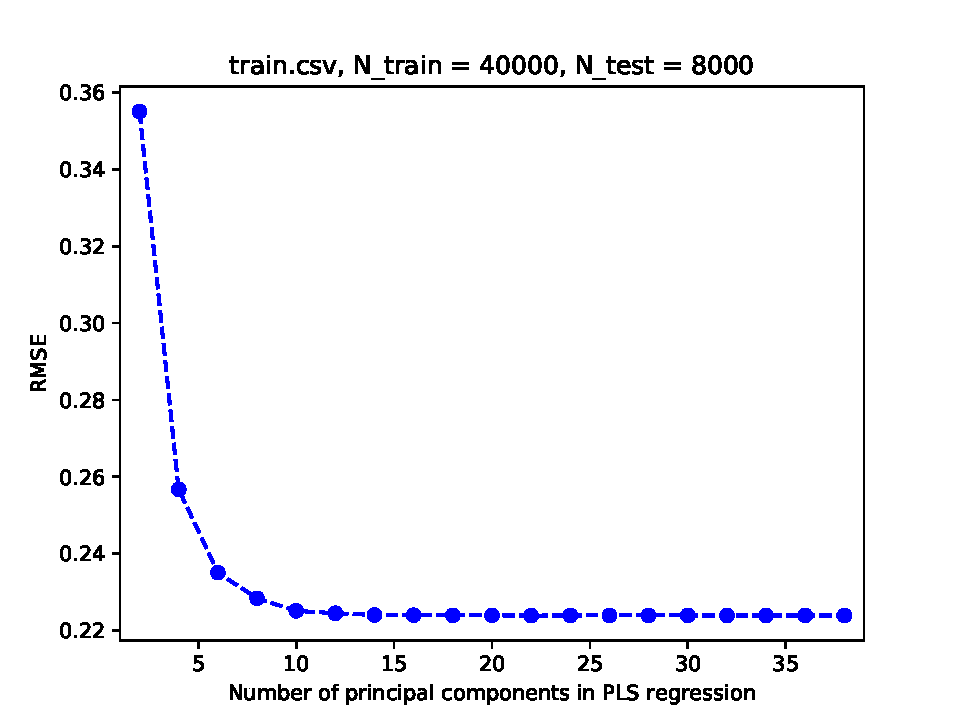
\includegraphics[width=\textwidth]{train_rdkit_N_train_40000_N_test_8000.pdf}
    \end{subfigure}
        \begin{subfigure}[!t]{0.2\textwidth}
        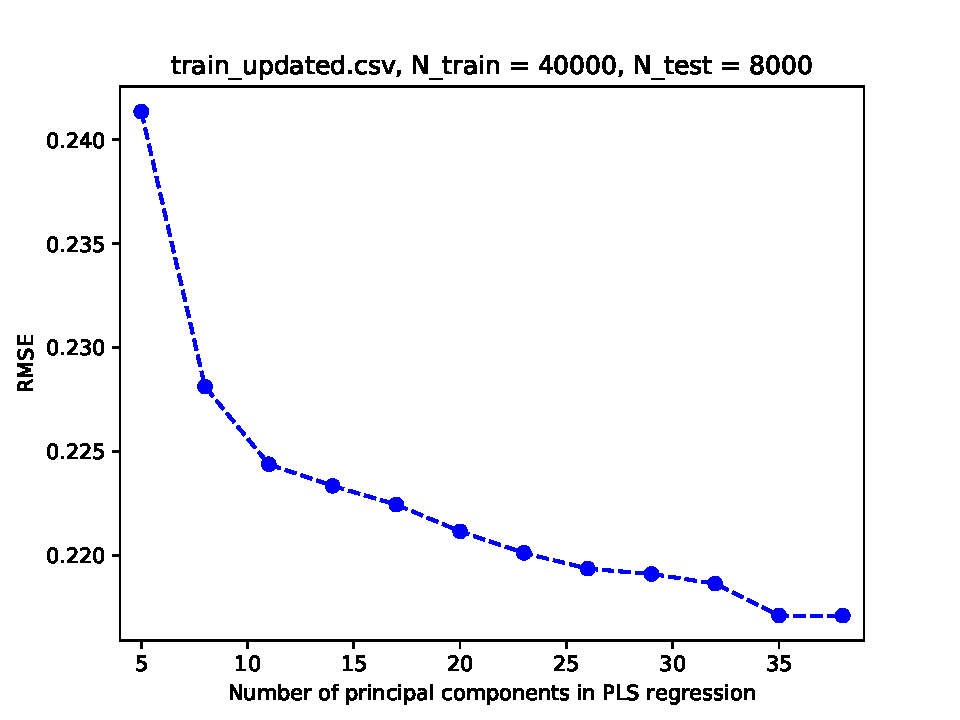
\includegraphics[width=\textwidth]{train_updated_N_train_40000_N_test_8000.pdf}
    \end{subfigure}
            \begin{subfigure}[!t]{0.2\textwidth}
        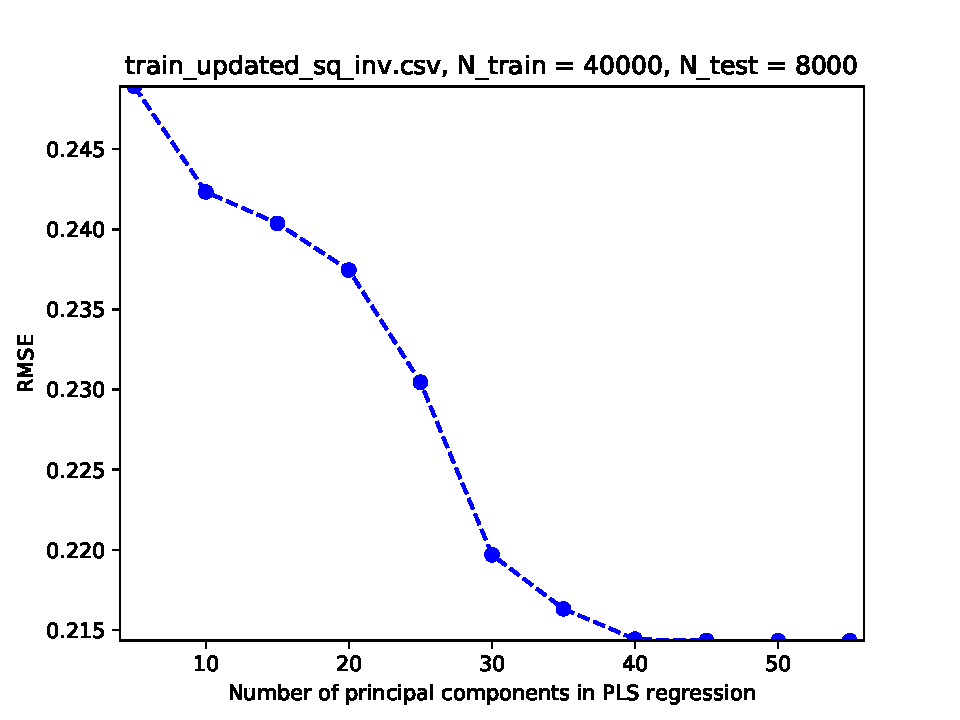
\includegraphics[width=\textwidth]{train_updated_sq_inv_N_train_40000_N_test_8000.pdf}
    \end{subfigure}\\
        \caption{(a) Results of PLS trained on the original data (no extra features). The RMSE is plotted as function of the number of principal components specified in the fitting. (b) Similar to (a), but but after adding rdkit features to the original data. (c) Similar to (a), but using the truncated dataset with chemistry features. (d) PLS on the truncated data set with additional features, their squares, inverses, and inverse squares. This is the best RMSE among our PLS attempts}
            \label{fig:PLS}
\end{figure}
\paragraph{}
Truncated data set with additional chemistry features produces improved results, shown in Fig. \ref{fig:PLS} (c), and the RMSE converges after ~30 components. This confirms to us that chemistry features do in fact provide new information not present in the original data. In order to introduce nonlinear terms to the data, we took squares, inverses and inverse squares of non-binary features. The reasoning is that the energy gap could be inversely proportional to one of the quantities. %For example, the Bohr atom energy is inversely proportional to the energy level number, although there is no direct analog to that in our features. 
The results of PLS applied to the data including the new powers of numeric features are shown in Fig. \ref{fig:PLS} (d). This approach yielded the lowest RMSE among all PLS methods. We also note that it takes 40 principal components for the RMSE to converge. This number is greater than that in (a) - (c), which means that the new components we added are in fact significant. We concluded that reducing the number of features was justified, and that there is some non-linearity present in the data.

\subsection{Multilayer Percetion (MLP) Regression}
\paragraph{}
We made a few attempts at using the MLPregressor from the sklearn neural network module to fit out data. We applied MLP to the original data as well as the truncated, feature-added data. In both cases, we saw an increase in RMSE with increasing number of hidden layers, with the minimum around 2-3 layers. In diagnosing the issue, we saw that the cross-validation loss would decrease rapidly at first and then stop changing, possibly trapped in a local minimum. Suspecting that we may not be finding the global minimum due to numerical issues, we have tried several steepest gradient descent-like methods, including a stochastic method with adaptive and constant step sizes. We then tried several activation functions, which penalize outliers differently. Finally, we tried to force the method to keep iterating by increasing the maximum number of iterations and decreasing the tolerance, with little success. 

\subsection{Decision Trees}
\paragraph{}
\textbf{Because of the discrete nature of the features, decision trees are ideal for predicting the gap values.} The final submission on Kaggle input is done by training a decision tree with maximum depth of 30. The choices of depth and maximum leaves have been explored and optimized based on testing, overtraining is avoided. Decision tree method is compared with the default linear regression, random forest, and a second order polynomial with ridge regression. The result is shown in Fig. \ref{fig:Prediction}. This testing RMSE score from the DT output is fairly close to the score on Kaggle.
\begin{figure}[] 
\centering
\begin{subfigure}[!t]{0.2\textwidth}
        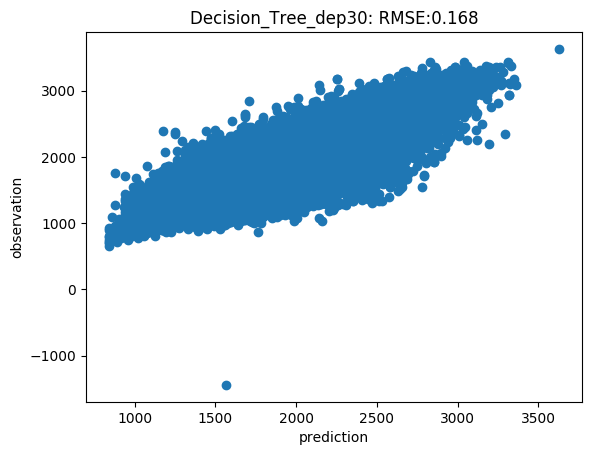
\includegraphics[width=\textwidth]{Decision_Tree_dep30_pred.png}
    \end{subfigure}
    \begin{subfigure}[!t]{0.2\textwidth}
        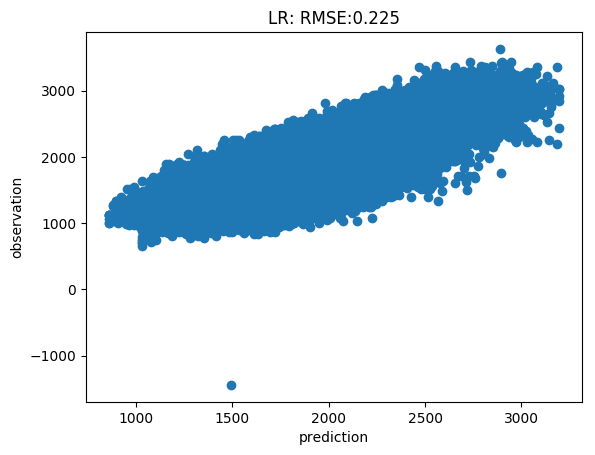
\includegraphics[width=\textwidth]{LR_pred.png}
    \end{subfigure}
        \begin{subfigure}[!t]{0.2\textwidth}
        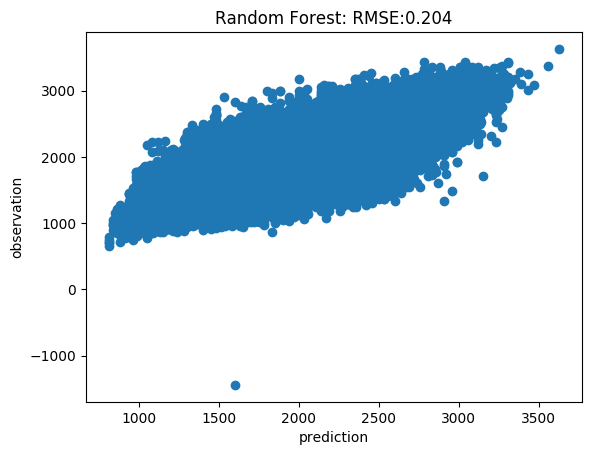
\includegraphics[width=\textwidth]{Random_Forest_pred.png}
    \end{subfigure}
            \begin{subfigure}[!t]{0.2\textwidth}
        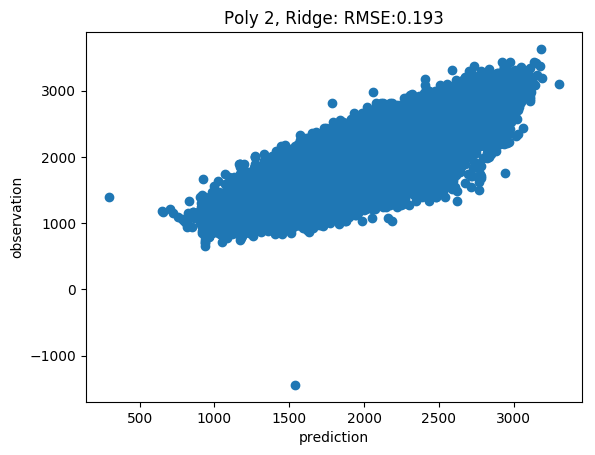
\includegraphics[width=\textwidth]{Poly_2_Ridge_pred.png}
    \end{subfigure}\\
        \caption{Results predicted gap value (x axis) and true gap value (y axis), with the RMSE labeled on title. (a) Decision Tree. (b) Linear Regression. (c) Random Forest. (d) Polynoimal.}
            \label{fig:Prediction}
\end{figure}


%\section{Methods: Validation (should we remove this?)}
%    \subsection{Split}
%In order to develop and validate our models quickly without having to submit them on kaggle, we used smaller subsets of our data (typically below 100,000 molecules) for testing models. We would use 20 percent of this subset as testing data, and the rest as training data. We would then study the error as function of the method used. 

\section{Discussion}
\paragraph{}
Given our results so far, the most promising direction to pursue is feature engineering: excluding insignificant features and adding new features made a significant improvement in our accuracy. In addition, methods that worked well involved some use of randomness or nonlinearity or both. These conclusions agree with an intuitive interpretation of the results in Fig. \ref{fig:PLS}. On the other hand, multilayer perception did not give immediate results. Given the time constraints, it is possible that we have not identified the correct neural net-like algorithm. With more time, we would pursue new features combined with better tuning of our models, most notably Random Forrest algorithms. Also, systematic uncertainties are not explored and it would be good to evaluate this in the future.

\end{document}

